\documentclass{report}

\input{~/dev/latex/template/preamble.tex}
\input{~/dev/latex/template/macros.tex}
\graphicspath{{./images}}

\title{\Huge{Chapter 1 Notes: Getting Started With Digital Media}}
\author{\huge{Nathan Warner}}
\date{\huge{Jan 27, 2023}}

\begin{document}
    \maketitle
    \begin{Large}
        \noindent \textbf{Learning Outcomes:}
    \end{Large}

    \bigbreak \noindent 
    \begin{enumerate}
        \item List the characteristics needed to become a skilled digital master.
        \item Identify how to name and save a file.
        \item Explain how to ensure digital security. 
        \item Practice the techniques for good keyboarding.
    \end{enumerate}

    \bigbreak \noindent \bigbreak \noindent \bigbreak \noindent 
    \begin{Large}
        \textbf{Key Terms:}
    \end{Large}

    \bigbreak \noindent 
    \begin{itemize}
        \item \textbf{Adware:} Software that displays unwanted advertisements 
        \item \textbf{Cyber Predator:} A person who uses the Internet to make contact with others (usually with children and teens) in order to harm them
        \item \textbf{Digital Media:} any com-bination of audio, video, images, and text used to convey a message through technology
        \item \textbf{Encryption:} Converting text into an unreadable series of numbers and let-ters to protect information. Digital encryption uses soft-ware that can scramble and unscramble the data
        \item \textbf{Ergonomics:} A science that studies the best way to design a workplace for maximum safety and productivity
        \item \textbf{Hacker:} A person who finds an electronic means of gain-ing unauthorized access to a computer.
        \item \textbf{Keylogger:} Software that tracks keyboard use and transmits it to be used for illegal purposes
        \item \textbf{Malware:} The abbrevia-tion for malicious software, designed to damage a com-puter or steal information.
        \item \textbf{Naming Convention:} A set of rules used in the naming of files and folders
        \item \textbf{Online Backup:} A means of backing up or storing data using the Internet.
        \item \textbf{Phising:} A social engi-neering activity where the perpetrator uses fake websites or emails to trick a user into providing personal information or passwords
        \item \textbf{Repetitive Stress Injury:} Muscle or joint injury that results from performing actions repeatedly.
        \item \textbf{Rootkit:} Type of malware that hides its presence on a computer
        \item \textbf{Server:} A computer designed to store files from multiple computers
        \item \textbf{Social Engineering:} Tricking users into providing information in the belief that a request is legitimate.
        \item \textbf{Spyware:} Software that gathers information about a user without their knowledge
        \item \textbf{Trojan:} Type of malware that disguises itself as legitimate software
        \item \textbf{Virus:} Type of malware that replicates itself and spreads to other computers
        \item \textbf{Worm:} Type of malware that also replicates itself but primarily spreads through networks
    \end{itemize}

    \pagebreak
    \begin{Large}
        \noindent \textbf{Key Concepts:}
    \end{Large}

    \bigbreak \noindent 
    \begin{itemize}
        \item The five commitments to learning include: be flexible, keep an open mind, use initiative, listen and read attentively, and seek to acquire new knowledge and skills. 
        \item The six behaviors that contribute to your ability to acquire a job and grow in the field of your choice include good attendance, promptness, proper attire, a clean and safe work environment, appropriate voice, and pride. 
        \item You can demonstrate your digital media skills by seeking certification from a secondary and/or post-secondary school or through a provider such as Adobe or Microsoft.
        \item Managing digital files is an essential part of creating a good work environment. 
        \item Strong passwords are those that meet a set of rules designed to make it difficult for others to figure out the word. 
        \item Repetitive stress injury (RSI) (including carpal tunnel syndrome) results from repeated movement of a particular part of the body.
    \end{itemize}

    \bigbreak \noindent \bigbreak \noindent \bigbreak \noindent  
    \begin{Large}
        \noindent \textbf{Commitment:}
    \end{Large}
    \bigbreak \noindent 
    In order to learn new software and computer skills, you must:

    \bigbreak \noindent 
    \begin{itemize}
        \item Be flexible
        \item Keep an open mind
        \item Use initiative
        \item Listen and read attentively
        \item Seek to acquire new knowledge and skills
    \end{itemize}

    \bigbreak \noindent \bigbreak \noindent \bigbreak \noindent 
    \begin{Large}
        \textbf{Work Skills For Multimedia Careers:}
    \end{Large}

    \bigbreak \noindent 
    \begin{itemize}
        \item Good attendance
        \item Promptness
        \item Proper attire
        \item Clean and safe work environment
        \item Appropriate voice
        \item Pride
    \end{itemize}


    \pagebreak
    \begin{Large}
       \noindent \textbf{Managing Files:} 
    \end{Large}
    
    \bigbreak \noindent 
    Digital media projects often include multiple components as part of the final product.
    These may include image, text, audio, and video files. All must be saved in such a way and in such a place that 
    anyone involved in the project can find the most current versions. 
    
    \bigbreak \noindent 
    \begin{Large}
        \textbf{Naming Files:}
    \end{Large}

    \bigbreak \noindent 
    The first step in managing files is deciding on a naming practice, or \textbf{ \textit{naming convention}}.
    Choose a name that clearly identifies the contents of the file. If files are to be shared, 
    the author's name or initials and some numbering method should be used to make 
    sure the correct versions are apparent.

    \bigbreak \noindent 
    If a filename includes multiple words, one of two formats should be used.

    \bigbreak \noindent 
    \begin{itemize}
        \item Link words with an underscore
        \item Link words with upper and lower case 
    \end{itemize}

    \bigbreak \noindent 
    Whitespace inbetween words should not be used because they can lead to problems down
    the road. They should especially be avoided in files that used in a web page because 
    the linking process replaces empty spaces with \%20, making the url address appear confusing when
    it is sited or referenced. 

    \bigbreak \noindent 
    \nt{Special symbols should also be avoided when naming files.}
    
    \bigbreak \noindent 
    \begin{Large}
        \textbf{Saving Files:}
    \end{Large}

    \bigbreak \noindent 
    You should also make sure save your files to the correct location. There should be a designated place to save project files, and everyone on a project
    team must know where that is.

    \bigbreak \noindent 
    Network locations or shared internet locations are often used to allow everyone
    access to the same material. Make sure you know where the shared folder is located. 
    Make sure you know what file type is adequate for the file you are working on. This is 
    especially important for image files. 

    \bigbreak \noindent 
    \nt{Make sure folder/file names are clearly identifiable.}  

    \bigbreak \noindent 
    \begin{Large}
        \textbf{Choosing Storage:}
    \end{Large}

    \bigbreak \noindent 
    Video and image files can often be very large, it is important to know
    what demands these files are making on your system.

    \bigbreak \noindent 
    Organizations often store files on dedicated serves. \textbf{Dedicated servers} are 
    one or more hard drives stored in a location seperate from the desktop computers used by 
    employees. While servers storage limits are usually much higher than standard desktops, 
    it is still important to take into consideration the size of the file that you are saving
    to the server.

    \bigbreak \noindent 
    \nt{Another means of storage can be a writeable CD or DVD.}

    \bigbreak \noindent 
    Flash drives are a means of storage that uses a circut board, unlike a hard drive 
    which uses a spinning plater. Because flash drives use a circut board, this means that there
    are no moving parts to break. Flash drives are attached to a computer through the usb port.
    This makes it easy to transfer data from one machine to another. 

    \bigbreak \noindent 
    \begin{Large}
        \textbf{Making Backups:}
    \end{Large}

    \bigbreak \noindent 
    There are 3 main ways of creating backups:

    \bigbreak \noindent 
    \begin{itemize}
        \item Backing up to a flash drive or another hard drive/external drive.
        \item \textbf{Online backup:} Files are transfered over the internet to a computer in a distant location.
        \item \textbf{Backup through the network:} Information is stored on another computer within the network.
    \end{itemize}

    \bigbreak \noindent 
    Short term, more frequent backups can be made to removable media such as flash drives.
    Long term backups may be sent to an online server.
    
    \bigbreak \noindent \bigbreak \noindent \bigbreak \noindent  
    \begin{Large}
        \textbf{Personal Security:}
    \end{Large}

    \bigbreak \noindent 
    It is important to protect yourself online. This means not revealing any personal
    information or providing information to sites that you do not trust.
    Online \textbf{ \textit{cyber predators}} who hunt for victims are dangerous to everyone. 
    Not everyone is as they appear online. Even the most seemingly harmless exchange 
    could lead to a dangerous situation.

    \bigbreak \noindent 
    Another danger is \textbf{ \textit{Identity Theft}}. This is an issue for 
    everyone who registers at websites, purchases items on the web, or uses social network
    sites. It is important to be aware of the more recent internet security issues. This 
    includes the latest \textbf{ \textit{Social Engineering}} scams or keylogging tricks.


    \bigbreak \noindent \bigbreak \noindent \bigbreak \noindent 
    \begin{Large}
        \textbf{Computer Security:}
    \end{Large}

    \bigbreak \noindent 
    Keeping your computer and network secure requires you to keep from dangers 
    such as \textbf{ \textit{Maleware}}. This is software that is downloaded on the
    victims computer without their knowledge, and with malicious intent.

    \bigbreak \noindent 
    \nt{It is important to understand the distinctions between each of the hazards.}

    \bigbreak \noindent 
    \begin{center}
       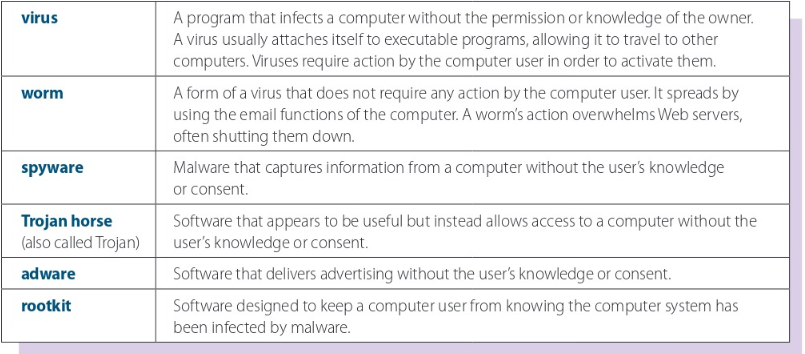
\includegraphics[scale=0.6]{ ./images/virus.png } 
    \end{center}

    \bigbreak \noindent 
    If you download software from the internet, make sure its from a secure site.
    You should also never open suspicious emails or unexpected attachments.

    \bigbreak \noindent 
    If you log into a public network, there is a potential risk to your computer. 
    Some networks are more secure than others, meaning they have passwords and \textbf{ \textit{encryption}}.
    Be careful what information you share over a network.
    
    \bigbreak \noindent 
    \nt{Remember that no software protection can prevent a network hacker from stealing information shared over an open network.}

    \bigbreak \noindent \bigbreak \noindent \bigbreak \noindent 
    \begin{Large}
        \textbf{Password Security:}
    \end{Large}
    
    \bigbreak \noindent 
    One of the most effective ways to keep your computer safe is through wise passwords. 
    If your password is easy to figure out, code hackers can easily gain access to
    your computer and its files. 

    \bigbreak \noindent 
    It is important for you password to have each of the following:

    \bigbreak \noindent 
    \begin{itemize}
        \item Have a minimum of eight characters
        \item Use both upper and lower case letters
        \item Use at least one number
        \item Use at least one special character
    \end{itemize}

    \bigbreak \noindent 
    \nt{ \textbf{ \textit{Phising}} is when hackers send out realistic emails asking for information}

    \bigbreak \noindent \bigbreak \noindent \bigbreak \noindent 
    \begin{Large}
        \textbf{Hardware Security:}
    \end{Large}

    \bigbreak \noindent 
    Because of the nature of portable laptops, they can be easily stolen. 
    Loss of the hardware is an obvious problem, but you also loose the information 
    that was stored on the machine. This is why it is important to make frequent backups 
    of your important data.

    \bigbreak \noindent 
    \nt{It is important that you pay attention to a situation that might compromise your machine.}

    \bigbreak \noindent \bigbreak \noindent \bigbreak \noindent 
    \begin{Large}
        \textbf{Acceptable use Policy (AUP)}
    \end{Large}
    
    \bigbreak \noindent 
    Organizations often use AUP's to encourage digital safety and appropriate use of hardware and software.
    These written agreements must be signed to ensure safety for everyone that is using the network.

    \bigbreak \noindent 
    These agreements may include the following:
    
    \bigbreak \noindent 
    \begin{itemize}
        \item Password selection requirements, including frequency of change.
        \item Software usage restriction.
        \item Netiquette rules, including prohibiton of inappropriate emailing or texting subjects.
        \item Limits on the use of systems or items that overtax the network.
    \end{itemize}
\end{document}

